\documentclass{beamer}

%% Use package -----------------------------------------------------------------

\usepackage[T1]{fontenc}
\usepackage[utf8]{inputenc}
\usepackage{lmodern}
\usepackage{graphicx}
\usepackage[absolute,overlay]{textpos}
\usepackage{multicol}
\usepackage{listings}
\usepackage{svg}

%% Beamer customization---------------------------------------------------------

\usepackage{xcolor}
\usetheme{Warsaw}

%% Themes
% Outer themes
\useoutertheme{shadow}
% Rounded boxes and shadows
\useinnertheme[shadow=true]{rounded}
% Solid \item symbols
\useinnertheme{circles}

%% Custom colors
\definecolor{rltgreen}{rgb}{0,0.5,0}
\definecolor{pasteur}{RGB}{0,90,154}
\setbeamerfont{block title}{size={}}
\setbeamercolor{structure}{fg=pasteur}
\setbeamercolor{item}{fg=pasteur}

%Color of title
\setbeamertemplate{frametitle}
{
    \nointerlineskip
    \begin{beamercolorbox}[sep=0.3cm,ht=1.8em,wd=\paperwidth]{frametitle}
        \vbox{}\vskip-2ex%
        \strut\insertframetitle\strut
        \vskip-0.8ex%
    \end{beamercolorbox}
}
% Hide navigation symbols
\setbeamertemplate{navigation symbols}{}

%% Title block
\setbeamercolor*{title}{use=structure,fg=white,bg=pasteur}

%% Bottom infolines
\setbeamertemplate{footline}
{
  \leavevmode%
  \hbox{%
  \begin{beamercolorbox}[wd=.3\paperwidth,ht=2.25ex,dp=1ex,center]{author in head/foot}%
    \usebeamerfont{author in head/foot}\insertshortauthor
  \end{beamercolorbox}%
  \begin{beamercolorbox}[wd=.7\paperwidth,ht=2.25ex,dp=1ex,center]{title in head/foot}%
    \usebeamerfont{title in head/foot}\insertshorttitle\hspace*{3em}
    \insertframenumber{} / \inserttotalframenumber\hspace*{1ex}
  \end{beamercolorbox}}%
  \vskip0pt%
}
\makeatletter

%% Top infolines
\setbeamertemplate{headline}{%
\leavevmode%
  \hbox{%
    \begin{beamercolorbox}[wd=\paperwidth,ht=2.5ex,dp=1.125ex]{palette quaternary}%
    \insertsectionnavigationhorizontal{\paperwidth}{}{\hskip0pt plus1filll}
    \end{beamercolorbox}%
  }
}

%% Define Snakemake ------------------------------------------------------------

\definecolor{eclipseBlue}{RGB}{42,0.0,255}
\definecolor{eclipseGreen}{RGB}{63,127,95}
\definecolor{eclipsePurple}{RGB}{127,0,85}

\lstset{language=Python}
\lstset{
    basicstyle=\tiny\ttfamily,
    morekeywords={rule, output, shell, params, run, configfile, temp},
    showstringspaces=false,
    commentstyle=\color{eclipseGreen}, % style of comments
    keywordstyle=\color{eclipsePurple}, % style of keywords
    stringstyle=\color{eclipseBlue}, % style of strings
}


%% Set up title ----------------------------------------------------------------

\title{Sequana: Motivations and Overview}
\author[T.Cokelaer \& D.Desvillechabrol]{Thomas Cokelaer and Dimitri Desvillechabrol}
\institute{Institut Pasteur}
\date{March 22d 2016}

\begin{document}

%% Title slide -----------------------------------------------------------------

\begin{frame}[plain]
    \titlepage
    \begin{textblock*}{5cm}(4.5cm,0.3cm)
        
\includegraphics[scale=0.09]{Institut_Pasteur.png}
    \end{textblock*}
\end{frame}

%% Slides ----------------------------------------------------------------------

\section{Motivation}

\begin{frame}
 \frametitle{NGS at Biomics}
 
 The Biomics Pole at Pasteur Institute is responsible for Next Generation Sequencing. Many aspects are covered including :
 
 \tiny
 \begin{block}{https://research.pasteur.fr/en/team/biomics/}
  \begin{itemize}
  \item De novo and targeted sequencing of viruses, prokaryotes and eukaryotes
  \item Variant (SNP, indel, large rearrangements) detection
  \item Human and Mouse SNP detection by array
  \item Transcriptional analysis (RNA-Seq) for both prokaryotes and eukaryotes
  \item 16S and deep-sequencing metagenomic studies (mouse, human, and other environments)
  \item Bottom-up whole proteomic analysis and quantification
  \item Analysis of a wide range of post-translational modifications
  \item Determination of the dynamics of protein complexes.
  \item Epigenetics (methylation studies)
  \item Projects involving two or more techniques (i.e. proteogenomics, single-cell DNA/RNA analysis)
  \end{itemize}
 \end{block}
 \small 
\pause
 We are developing NGS pipelines like many others and have started to gather
tools and information in a common repository called \textbf{Sequana}.
\end{frame}



\begin{frame}
 \frametitle{Needs}
 
    \begin{block}{What do we have \dots or not ?}
     
\includegraphics[scale=0.05]{positive.png}\; A bunch of pipelines dedicated to NGS data\\
     
\includegraphics[scale=0.05]{positive.png}\; Expertise\\
     
\includegraphics[scale=0.05]{negative.png}\; Lack of \\
	\begin{itemize}
	 \item traceability ?
	 \item reproducibility ? 
	 \item co-development ? 
	 \item common framework ?
	\end{itemize}
    \end{block}
    
    \begin{block}{What do we need ?}
    \begin{itemize}
     \item A framework to combine or re-use existing pipelines
     \item Fast development (iterative process)
     \item Continuous Integration and Quality Software (reproducibility, traceability, test, documentation)
    \end{itemize}
    \end{block}


 
\end{frame}
\section{Sequana package}


\begin{frame}
    \frametitle{Why Sequana ?}
    
    \begin{block}{Enforce a common framework}
    \begin{itemize}
        \item Using Snakemake as a common language to design new pipelines
        \item Provide reusable snakemake rules
    \end{itemize} 
     \end{block}

    \begin{block}{A common entry point to }
    \begin{itemize}
        \item Share information
        \item Share pipelines
        \item Share Code
    \end{itemize} 
    \end{block}

    \begin{block}{Synergy to help on }
    \begin{itemize}
        \item Software Quality
        \item Diffusion
        \item Teaching
    \end{itemize} 
    \end{block}
    
\end{frame}

\begin{frame}[fragile]
    \frametitle{Pipelines included}
    
    \begin{block}{Snakefile}
    Snakefile are stored in directories called pipelines and accessible by name in Python
    \begin{lstlisting}
     >>> from sequana import snakemake
     >>> snakemake.rules.keys()
     ['dag', 'biomics', 'variant']
     >>> snakemake.rules['variants']
    '/home/cokelaer/Work/github/sequana/pipelines/variants/Snakefile'
    \end{lstlisting}

    It is therefore easy to include them in your own Snakefile:
    \begin{lstlisting}
    import sequana.snakemake as sm
    include: sm.rules['dag']
    include: sm.rules['variants']
    \end{lstlisting}

    \end{block}
\end{frame}

\begin{frame}[fragile]
    \frametitle{Report}
    
    We will provide a system of HTML reporting using sequana and JINJA templating
    \begin{block}{Snakefile}
    \begin{lstlisting}
    rule report:
    input:
        dag = "dag.svg"
    output: "report/index.html"
    run:
        from sequana import report_main
        s = report_main.SequanaReport()
        s.create_report()
        shell("cp Snakefile report/")
        shell("cp dag.svg report/")    
    \end{lstlisting}
    \end{block}
\end{frame}


\begin{frame}[fragile]
    \frametitle{Utilities}
    
    \footnotesize
    In addition to pipelines and reports, multi-purpose codes can be included within Sequana. 
    We currently have some tools to handle BAM, FastQ but tend to rely on existing packages such as pysam and pyVCF.
    Here is a simple function that retrieves the flags of a BAM file into a Pandas DataFrame
    
    \begin{block}{Snakefile}
    \begin{lstlisting}
    >>> # BAM is a class that inherits from pysam.Alignment and 
    >>> # add a couple of functions
    >>> from sequana import BAM
    >>> b = BAM("filename.bam")
    >>> df = b.get_flags_as_df()
    >>> df.sum()
    1       1526795
    2          2703
    4       1523785
    8       1523785
    16         1513
    32         1513
    64       763395
    128      763400
    256          13
    512           0
    1024          0
    2048          0
    dtype: int64
    \end{lstlisting}
    \end{block}
\end{frame}


\section{Code}

\begin{frame}[fragile]
    \frametitle{High code quality}
    \begin{block}{}
    Continuous Integration on Travis with currently 50\% coverage
    \end{block}
    
    
    %\begin{textblock*}{7cm}(.5cm,3.5cm)
        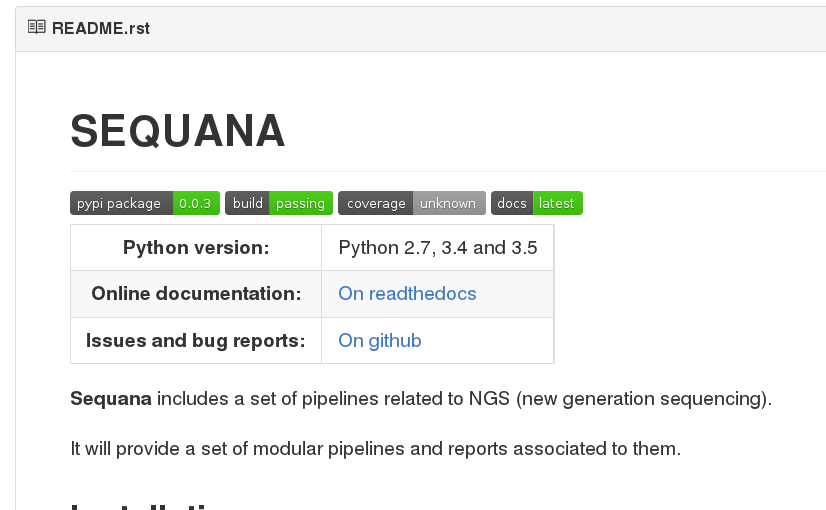
\includegraphics[scale=0.35]{sequana_quality.png}
    %\end{textblock*}
\end{frame}

\begin{frame}[fragile]

Open the file report/index.html for example of the current report (v0.0.3)

\end{frame}


\section{Contributions}
\begin{frame}{How to contribute ?}
\begin{enumerate}
 \item transform existing pipelines into Snakefiles and add them to Sequana.
 \item Identify parts that can be transformed into modules
 \item add tests
 \item Benchmarks ?
 \item complete documentation
 \item Add data processing or visualisation tools 
 \item Other ideas welcome
 \end{enumerate}
\end{frame}



\section{Summary}

\begin{frame}[fragile]
  \begin{block}{Summary}
    \begin{itemize}
      \item Sequana is used at biomics to share NGS pipelines (currently variants and fix contamination)
      \item Ease design of new pipelines. 
      \item Single entry point
      \item share expertise and existing pipelines
      \item automatic reports
      \item reaching a high quality and trustable code
    \end{itemize}
   \end{block}
 
  \begin{block}{Links}
    \begin{itemize}
      \item Join the github  : https://github.com/sequana/sequana    
      \item Doc on line on sequana.readthedocs.org
    \end{itemize}
  \end{block}
\end{frame}


\end{document}
